\documentclass{article}
\usepackage[utf8]{inputenc}
\usepackage{graphicx}
\usepackage{ragged2e}
\usepackage[margin=2.5cm]{geometry}
\usepackage{array}
\usepackage{wrapfig}
\usepackage{multirow}
\usepackage{rotating}
\usepackage{tikz}
\usepackage{tabularx}
\usepackage{amsmath}
\usepackage{wrapfig}
\usepackage{mathtools}
\usepackage[table]{xcolor}
\usepackage{multirow}
\usepackage{polski}
\usepackage{float}
\usepackage{rotating}
\usepackage{natbib}
\usepackage{matlab-prettifier}
\usepackage{graphicx}
\usepackage[dvipsnames]{xcolor}
\usepackage{amssymb}
\usepackage[export]{adjustbox}
% AAAAAAAAAAAAAAAAAAAAAAAAAAAAAAAAAAAAAAAAAAAAAAAAAA
% AAAAAAAAAAAAAAAAAAAAAAAAAAAAAAAAAAAAAAAAAAAAAAAAAA
% AAAAAAAAAAAAAAAAAAAAAAAAAAAAAAAAAAAAAAAAAAAAAAAAAAAAAAAAAAAAAAAAAAAAAAAAAAAAAAAAAAAAAAAAAAAAAAAAAAAAAAAAAAAAAAAAAAAAAAAAAAAAAAAAAAAAAAAAAAAAAAAAAAAAAAAAAAAAAAAAAAAAAAAAAAAAAAAAAAAAAAAAAAAAAAAAAAAAAAAAAAAAAAAAAAAAAAAAAAAAAAAAAAAAAAAAAAAAAAAAAAAAAAAAAAAAAAAAAAAAAAAAAAAAAAAAAAAAAAAAAAAAAAAAAAAAAAAAAAAAAAAAAAAAAAAAAAAAAAAAAAAAAAAAAAAAAAAAAAAAAAAAAAAAAAAAAAAAAAAAAAAAAAAAAAAAAAAAAAAAAAAAAAAAAAAAAAAAAAAAAAAAAAAAAAAAAAAAAAAAAAAAAAAAAAAAAAAAAAAAAAAAAAAAAAAAAAAAAAAAAAAAAAAAAAAAAAAAAAAAAAAAAAAAAAAAAAAAAAAAAAAAAAAAAAAAAAAAAAAAAAAAAAAAAAAAAAAAAAAAAAAAAAAAAAAAAAAAAAAAAAAAAAAAAAAAAAAAAAAAAAAAAAAAAAAAAAAAAAAAAAAAAAAAAAAAAAAAAAAAAAAAAAAAAAAAAAAAAAAAAAAAAAAAAAAAAAAAAAAAAAAAAAAAAAAAAAAAAAAAAAAAAAAAAAAAAAAAAAAA
% AAAAAAAAAAAAAAAAAAAAAAAAAAAAAAAAAAAAAAAAAAAAAAAAAAAAAAAAAAAAAAAAAAAAAAAAAAAAAAAAAAAAAAAAAAAAAAAAAAAAAAAAAAAAAAAAAAAAAAAAAAAAAAAAAAAAAAAAAAAAAAAAAAAAAAAAAAAAAAAAAAAAAAAAAAAAAAAAAAAAAAAAAAAAAAAAAAAAAAAAAAAAAAAAAAAAAAAAAAAAAAAAAAAAAAAAAAAAAAAAAAAAAAAAAAAAAAAAAAAAAAAAAAAAAAAAAAAAAAAAAAAAAAAAAAAAAAAAAAAAAAAAAAAAAAAAAAAAAAAAAAAAAAAAAAAAAAAAAAAAAAAAAAAAAAAAAAAAAAAAAAAAAAAAAAAAAAAAAAAAAAAAAAAAAAAAAAAAAAAAAAAAAAAAAAAAAAAAAAAAAAAAAAAAAAAAAAAAAAAAAAAAAAAAAAAAAAAAAAAAAAAAAAAAAAAAAAAAAAAAAAAAAAAAAAAAAAAAAAAAAAAAAAAAAAAAAAAAAAAAAAAAAAAAAAAAAAAAAAAAAAAAAAAAAAAAAAAAAAAAAAAAAAAAAAAAAAAAAAAAAAAAAAAAAAAAAAAAAAAAAAAAAAAAAAAAAAAAAAAAAAAAAAAAAAAAAAAAAAAAAAAAAAAAAAAAAAAAAAAAAAAAAAAAAAAAAAAAAAAAAAAAAAAAAAAAAAAAAAAAAAAAAAAAAAAAAAAAAAAAAAAAAAAAAAAAAAAAAAAAAAAAAAAAAAAAAAAAAAAAAAAAAAAAAAAAAAAAAAAAAAAAAAAAAAAAAAAAAAAAAAAAAAAAAAAAAAAAAAAAAAAAAAAAAAAAAAAAAAAAAAAAAAAAAAAAAAAAAAAAAAAAAAAAAAAAAAAAAAAAAAAAAAAAAAAAAAAAAAAAAAAAAAAAAAAAAAAAAAAAAAAAAAAAAAAAAAAAAAAAAAAAAAAAAAAAAAAAAAAAAAAAAAAAAAAAAAAAAAAAAAAAAAAAAAAAAAAAAAAAAAAAAAAAAAAAAAAAAAAAAAAAAAAAAAAAAAAAAAAAAAAAAAAAAAAAAAAAAAAAAAAAAAAAAAAAAAAAAAAAAAAAAAAAAAAAAAAAAAAAAAAAAAAAAAAAAAAAAAAAAAAAAAAAAAAAAAAAAAAAAAAAAAAAAAAAAAAAAAAAAAAAAAAAAAAAAAAAAAAAAAAAAAAAAAAAAAAAAAAAAAAAAAAAAAAAAAAAAAAAAAAAAAAAAAAAAAAAAAAAAAAAAAAAAAAAAAAAAAAAAAAAAAAAAAAAAAAAAAAAAAAAAAAAAAAAAAAAAAAAAAAAAAAAAAAAAAAAAAAAAAAAAAAAAAAAAAAAAAAAAAAAAAAAAAAAAAAAAAAAAAAAAAAAAAAAAAAAAAAAAAAAAAAAAAAAAAAAAAAAAAAAAAAAAAAAAAAAAAAAAAAAAAAAAAAAAAAAAAAAAAAAAAAAAAAAAAAAAAAAAAAAAAAAAAAAAAAAAAAAAAAAAAAAAAAAAAAAAAAAAAAAAAAAAAAAAAAAAAAAAAAAAAAAAAAAAAAAAAAAAAAAAAAAAAAAAAAAAAAAAAAAAAAAAAAAAAAAAAAAAAAAAAAAAAAAAAAAAAAAAAAAAAAAAAAAAAAAAAAAAAAAAAAAAAAAAAAAAAAAAAAAAAAAAAAAAAAAAAAAAAAAAAAAAAAAAAAAAAAAAAAAAAAAAAAAAAAAAAAAAAAAAAAAAAAAAAAAAAAAAAAAAAAAAAAAAAAAAAAAAAAAAAAAAAAAAAAAAAAAAAAAAAAAAAAAAAAAAAAAAAAAAAAAAAAAAAAAAAAAAAAAAAAAAAAAAAAAAAAAAAAAAAAAAAAAAAAAAAAAAAAAAAAAAAAAAAAAAAAAAAAAAAAAAAAAAAAAAAAAAAAAAAAAAAAAAAAAAAAAAAAAAAAAAAAAAAAAAAAAAAAAAAAAAAAAAAAAAAAAAAAAAAAAAAAAAAAAAAAAAAAAAAAAAAAAAAAAAAAAAAAAAAAAAAAAAAAAAAAAAAAAAAAAAAAAAAAAAAAAAAAAAAAAAAAAAAAAAAAAAAAAAAAAAAAAAAAAAAAAAAAAAAAAAAAAAAAAAAAAAAAAAAAAAAAAAAAAAAAAAAAAAAAAAAAAAAAAAAAAAAAAAAAAAAAAAAAAAAAAAAAAAAAAAAAAAAAAAAAAAAAAAAAAAAAAAAAAAAAAAAAAAAAAAAAAAAAAAAAAAAAAAAAAAAAAAAAAAAAAAAAAAAAAAAAAAAAAAAAAAAAAAAAAAAAAAAAAAAAAAAAAAAAAAAAAAAAAAAAAAAAAAAAAAAAAAAAAAAAAAAAAAAAAAAAAAAAAAAAAAAAAAAAAAAAAAAAAAAAAAAAAAAAAAAAAAAAAAAAAAAAAAAAAAAAAAAAAAAAAAAAAAAAAAAAAAAAAAAAAAAAAAAAAAAAAAAAAAAAAAAAAAAAAAAAAAAAAAAAAAAAAAAAAAAAAAAAAAAAAAAAAAAAAAAAAAAAAAAAAAAAAAAAAAAAAAAAAAAAAAAAAAAAAAAAAAAAAAAAAAAAAAAAAAAAAAAAAAAAAAAAAAAAAAAAAAAAAAAAAAAAAAAAAAAAAAAAAAAAAAAAAAAAAAAAAAAAAAAAAAAAAAAAAAAAAAAAAAAAAAAAAAAAAAAAAAAAAAAAAAAAAAAAAAAAAAAAAAAAAAAAAAAAAAAAAAAAAAAAAAAAAAAAAAAAAAAAAAAAAAAAAAAAAAAAAAAAAAAAAAAAAAAAAAAAAAAAAAAAAAAAAAAAAAAAAAAAAAAAAAAAAAAAAAAAAAAAAAAAAAAAAAAAAAAAAAAAAAAAAAAAAAAAAAAAAAAAAAAAAAAAAAAAAAAAAAAAAAAAAAAAAAAAAAAAAAAAAAAAAAAAAAAAAAAAAAAAAAAAAAAAAAAAAAAAAAAAAAAAAAAAAAAAAAAAAAAAAAAAAAAAAAAAAAAAAAAAAAAAAAAAAAAAAAAAAAAAAAAAAAAAAAAAAAAAAAAAAAAAAAAAAAAAAAAAAAAAAAAAAAAAAAAAAAAAAAAAAAAAAAAAAAAAAAAAAAAAAAAAAAAAAAAAAAAAAAAAAAAAAAAAAAAAAAAAAAAAAAAAAAAAAAAAAAAAAAAAAAAAAAAAAAAAAAAAAAAAAAAAAAAAAAAAAAAAAAAAAAAAAAAAAAAAAAAAAAAAAAAAAAAAAAAAAAAAAAAAAAAAAAAAAAAAAAAAAAAAAAAAAAAAAAAAAAAAAAAAAAAAAAAAAAAAAAAAAAAAAAAAAAAAAAAAAAAAAAAAAAAAAAAAAAAAAAAAAAAAAAAAAAAAAAAAAAAAAAAAAAAAAAAAAAAAAAAAAAAAAAAAAAAAAAAAAAAAAAAAAAAAAAAAAAAAAAAAAAAAAAAAAAAAAAAAAAAAAAAAAAAAAAAAAAAAAAAAAAAAAAAAAAAAAAAAAAAAAAAAAAAAAAAAAAAAAAAAAAAAAAAAAAAAAAAAAAAAAAAAAAAAAAAAAAAAAAAAAAAAAAAAAAAAAAAAAAAAAAAAAAAAAAAAAAAAAAAAAAAAAAAAAAAAAAAAAAAAAAAAAAAAAAAAAAAAAAAAAAAAAAAAAAAAAAAAAAAAAAAAAAAAAAAAAAAAAAAAAAAAAAAAAAAAAAAAAAAAAAAAAAAAAAAAAAAAAAAAAAAAAAAAAAAAAAAAAAAAAAAAAAAAAAAAAAAAAAAAAAAAAAAAAAAAAAAAAAAAAAAAAAAAAAAAAAAAAAAAAAAAAAAAAAAAAAAAAAAAAAAAAAAAAAAAAAAAAAAAAAAAAAAAAAAAAAAAAAAAAAAAAAAAAAAAAAAAAAAAAAAAAAAAAAAAAAAAAAAAAAAAAAAAAAAAAAAAAAAAAAAAAAAAAAAAAAAAAAAAAAAAAAAAAAAAAAAAAAAAAAAAAAAAAAAAAAAAAAAAAAAAAAAAAAAAAAAAAAAAAAAAAAAAAAAAAAAAAAAAAAAAAAAAAAAAAAAAAAAAAAAAAAAAAAAAAAAAAAAAAAAAAAAAAAAAAAAAAAAAAAAAAAAAAAAAAAAAAAAAAAAAAAAAAAAAAAAAAAAAAAAAAAAAAAAAAAAAAAAAAAAAAAAAAAAAAAAAAAAAAAAAAAAAAAAAAAAAAAAAAAAAAAAAAAAAAAAAAAAAAAAAAAAAAAAAAAAAAAAAAAAAAAAAAAAAAAAAAAAAAAAAAAAAAAAAAAAAAAAAAAAAAAAAAAAAAAAAAAAAAAAAAAAAAAAAAAAAAAAAAAAAAAAAAAAAAAAAAAAAAAAAAAAAAAAAAAAAAAAAAAAAAAAAAAAAAAAAAAAAAAAAAAAAAAAAAAAAAAAAAAAAAAAAAAAAAAAAAAAAAAAAAAAAAAAAAAAAAAAAAAAAAAAAAAAAAAAAAAAAAAAAAAAAAAAAAAAAAAAAAAAAAAAAAAAAAAAAAAAAAAAAAAAAAAAAAAAAAAAAAAAAAAAAAAAAAAAAAAAAAAAAAAAAAAAAAAAAAAAAAAAAAAAAAAAAAAAAAAAAAAAAAAAAAAAAAAAAA
% https://i.ytimg.com/vi/gz5hy_F75QM/hqdefault.jpg
% https://www.youtube.com/watch?v=gz5hy_F75QM
\title{Miniprojekt}
\author{AUTOR}
\date{}

\definecolor{mygreen}{rgb}{0.0, 0.5, 0.0}
\newcommand{\inv}{^{\raisebox{.2ex}{$\scriptscriptstyle-1$}}}
\begin{document}

\maketitle

\section{Wstęp}
\begin{figure}[h!]
    \centering
    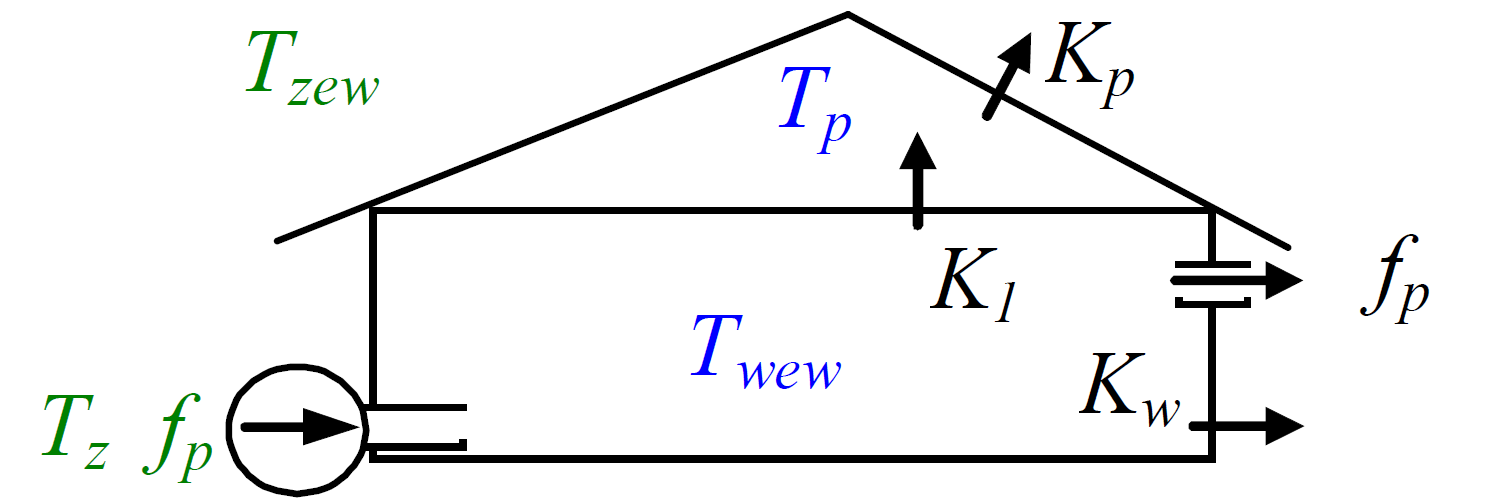
\includegraphics[scale=0.2]{domek_rysunek.png}
    \caption{Przykład z ogrzewaniem przez nawiew}
    \label{fig:domek_rysunek}
\end{figure}
\\Oto nieliniowy model obiektu:

\[\begin{cases}
    C_{vw} \dot{T}_{wew}(t) = c_{p}\rho_{p}f_{p}(t)\Big( T_{z}(t)-T_{wew}(t)\Big)-K_{1} \Big(T_{wew}(t)-T_{p}(t)\Big)-K_{w}\Big( T_{wew}(t)-T_{zew}(t)\Big)      \\
    C_{vp} \dot{T}_{p}(t)=K_{1}\Big( T_{wew}(t)-T_{p}(t)\Big)-K_{p}\Big( T_{p}(t)-T_{zew}(t)\Big)  
\end{cases}\]

\begin{flushleft}
    Właściwości modelu i ich wartości nominalne zadane podczas zajęć:
\end{flushleft}{}

\begin{itemize}
    \item Wymiary budynku, który zakładamy, że jest prostopadłościanem z ostrosłupem jako poddasze
    \begin{itemize}
        \item[] $dl = 20 m$ - długość budynku
        \item[] $szer = 10 m$ -szerokość budynku
        \item[] $h_{wew}=5 m$ - wysokość wnętrza
        \item[] $h_{p}=1.5 m$ - wysokość poddasza
        \item[] $V_{wew}=dl\cdot szer\cdot h_{w}=1000 m^{3}$ - Objętość wnętrza
        \item[] $V_{p}=\frac{dl\cdot szer\cdot h_{p}}{3}=100 m^{3}$ - Objętość poddasza
    \end{itemize}{}


    \item Zmienne stanu
    \begin{itemize}
    \color{blue}
        \item[] $T_{wewN} = 21^{\circ}C$ - Nominalna temperatura wewnętrzna 
        \item[] $T_{pN}=19^{\circ}C$ - Nominalna temperatura poddasza
    \end{itemize}

    
    
    \color{black}
    \item Zmienne wejściowe
    \begin{itemize}
    \color{mygreen}
        \item[] $T_{zewN} = -1^{\circ}C$ - Nominalna temperatura na zewnątrz
        \item[] $T_{zN}=24^{\circ}C$ - Nominalna temperatura powietrza
        \item[] $f_{pN}=1 \frac{m^{3}}{s}$ - Nominalne wdmuchiwane powietrze
    \end{itemize}
    
    
\newpage
    \item Inne parametry modelu
    \begin{itemize}
        \color{black}
        \item[] $\rho_{p}=1.2 \frac{kg}{m^3}$ - gęstość powietrza
        \item[] $c_{p}=1000\frac{J}{kg\cdot ^{\circ}C}$ - ciepło
        \item[] $C_{vw}=c_{p}\cdot \rho_{p} \cdot V_{w}=1200000\frac{J}{^{\circ}C}$ - pojemność cieplna
        \item[] $C_{vp}=c_{p}\cdot \rho_{p} \cdot V_{p}=120000\frac{J}{^{\circ}C}$ - pojemność cieplna
    \end{itemize}


    \item Współczynniki przenikalności cieplnej
    \begin{itemize}
        \item[] $K_{1}=? \frac{W}{^{\circ}C}$ - z wnętrza na poddasze 
        \item[] $K_{w}=? \frac{W}{^{\circ}C}$ - z wnętrza na zewnątrz
        \item[] $K_{p}=0.25\cdot K_{w}=? \frac{W}{^{\circ}C}$ - z poddasza na zewnątrz 
    \end{itemize}
\end{itemize}

Współczynniki K należy obliczyć podstawiając za pochodne zera, a za pozostałe wartości znane nam wartości nominalne. Otrzymujemy takie oto równanie:
\\ \\
% %%%%%%%%%%%%%%%%%%%%%%%%%%%%%%%%%%%%%%%%%%%%%%%%%%%%%%%%%%%%%%%%%%%%%%%%%%%%%
Rozwiązanie Analityczne: 
\[\begin{cases}
     K_{w} =\frac{c_{p}\rho_{p}f_{pN}\Big( T_{zN}-T_{wewN}\Big)}{0.25\cdot \Big( T_{pN}-T_{zewN}\Big) \ +\Big( T_{wewN}-T_{zewN}\Big)}     \\
    K_{1}=\frac{0.25\cdot K_{w}\Big( T_{pN}-T_{zewN}\Big)}{\Big( T_{wewN}-T_{pN}\Big)} 
\end{cases}\]

% %%%%%%%%%%%%%%%%%%%%%%%%%%%%%%%%%%%%%%%%%%%%%%%%%%%%%%%%%%%%%%%%%%%%%%%%%%%%%
\begin{flushleft}
    
Rozwiązanie Macierzowe:
\end{flushleft}{}

% \begin{equation}
\begin{center}
% \begin{flushleft}

    \begin{bmatrix}
        K_{1} \\[0.3em]
        K_{w}           
    \end{bmatrix}
    =
$
\begin{bmatrix}
    \left(T_{wewN}-T_{pN}\right) & \left( T_{wewN}-T_{zewN}\right)  \\[0.3em]
    \left( T_{wewN}-T_{pN}\right) & -0.25\left( T_{pN}-T_{zewN
    }\right)          
\end{bmatrix}^{-1}
$
    \begin{bmatrix}
        c_{p}\rho_{p}f_{pN}\Big( T_{zN}-T_{wewN}\Big) \\[0.3em]
        0            
    \end{bmatrix}
\end{center}
% \end{flushleft}{}
% %%%%%%%%%%%%%%%%%%%%%%%%%%%%%%%%%%%%%%%%%%%%%%%%%%%%%%%%%%%%%%%%%%%%%%%%%%%%%
Wyliczone współczynniki K:
\vspace{-5ex}
\begin{center}
    \[\begin{cases}
        K_{1}\approx 333.33  \frac{W}{^{\circ}C} \\
        K_{w}\approx 133.33  \frac{W}{^{\circ}C} \\
        K_{p}=0.25\cdot K_{w}\approx 33.33 \frac{W}{^{\circ}C}
    \end{cases}\]
\end{center}
% \end{equation}
% %%%%%%%%%%%%%%%%%%%%%%%%%%%%%%%%%%%%%%%%%%%%%%%%%%%%%%%%%%%%%%%%%%%%%%%%%%%%%
% Warunki poczatkowe dla syulacji w state space
% wartosci poczatkowe2
\\
Warunki początkowe:
\[\begin{cases}
    T_{wew0} = \frac{(c_{p}\cdot \rho_{p} \cdot f_{p}\cdot T_{z}+K_{1}\cdot K_{p}\cdot T_{zew}\cdot (K_{1}+K_{p}) +K_{w}\cdot T_{zew})}{(c_{p}\cdot \rho_{p}\cdot f_{p}+K_{1}+K_{w}-(K_{1}^{2})\cdot (K_{1}+K_{p}))}  \\
    T_{p0} = (K_{1}\cdot T_{wew0}+K_{p}\cdot T_{zew})\cdot (K_{1}+K_{p})
\end{cases}\]
% %%%%%%%%%%%%%%%%%%%%%%%%%%%%%%%%%%%%%%%%%%%%%%%%%%%%%%%%%%%%%%%%%%%%%%%%%%%%%
\\

Następnie na podstawie równań konstruujemy trzy modele w simulinku. Pierwszym z nich jest model nieliniowy:

\begin{figure}
    \centering
    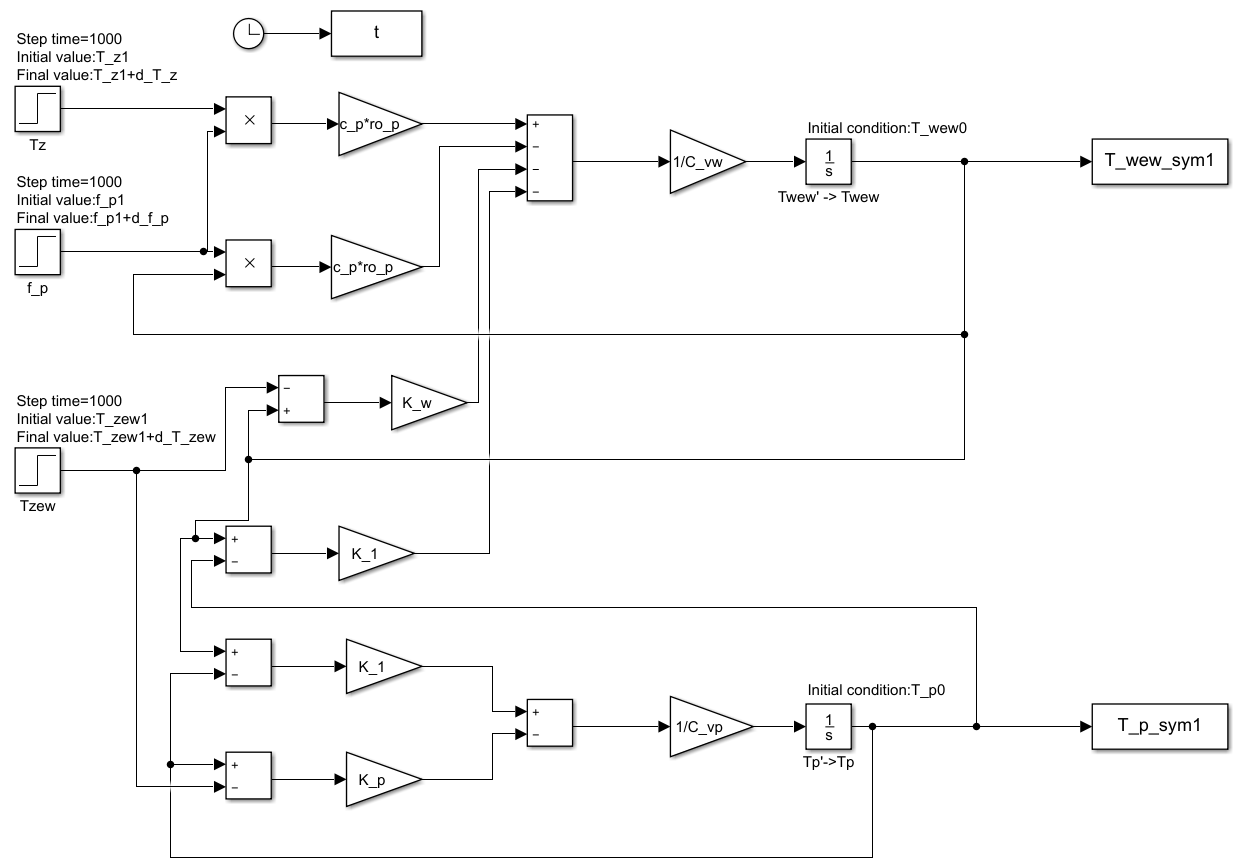
\includegraphics[scale=0.33]{model_bloki.png}
    \caption{Schemat Modelu Nieliniowego}
    \label{model:NL}
\end{figure}
% %%%%%%%%%%%%%%%%%%%%%%%%%%%%%%%%%%%%%%%%%%%%%%%%%%%%%%%%%%%%%%%%%%%%%%%%%%%%%% 
\newpage
\section{Charakterystyki statyczne}

Charakterystyki styczne z zaznaczonymi na czerwono punktami nominalnymi:

\begin{figure}[h!]
    \centering
    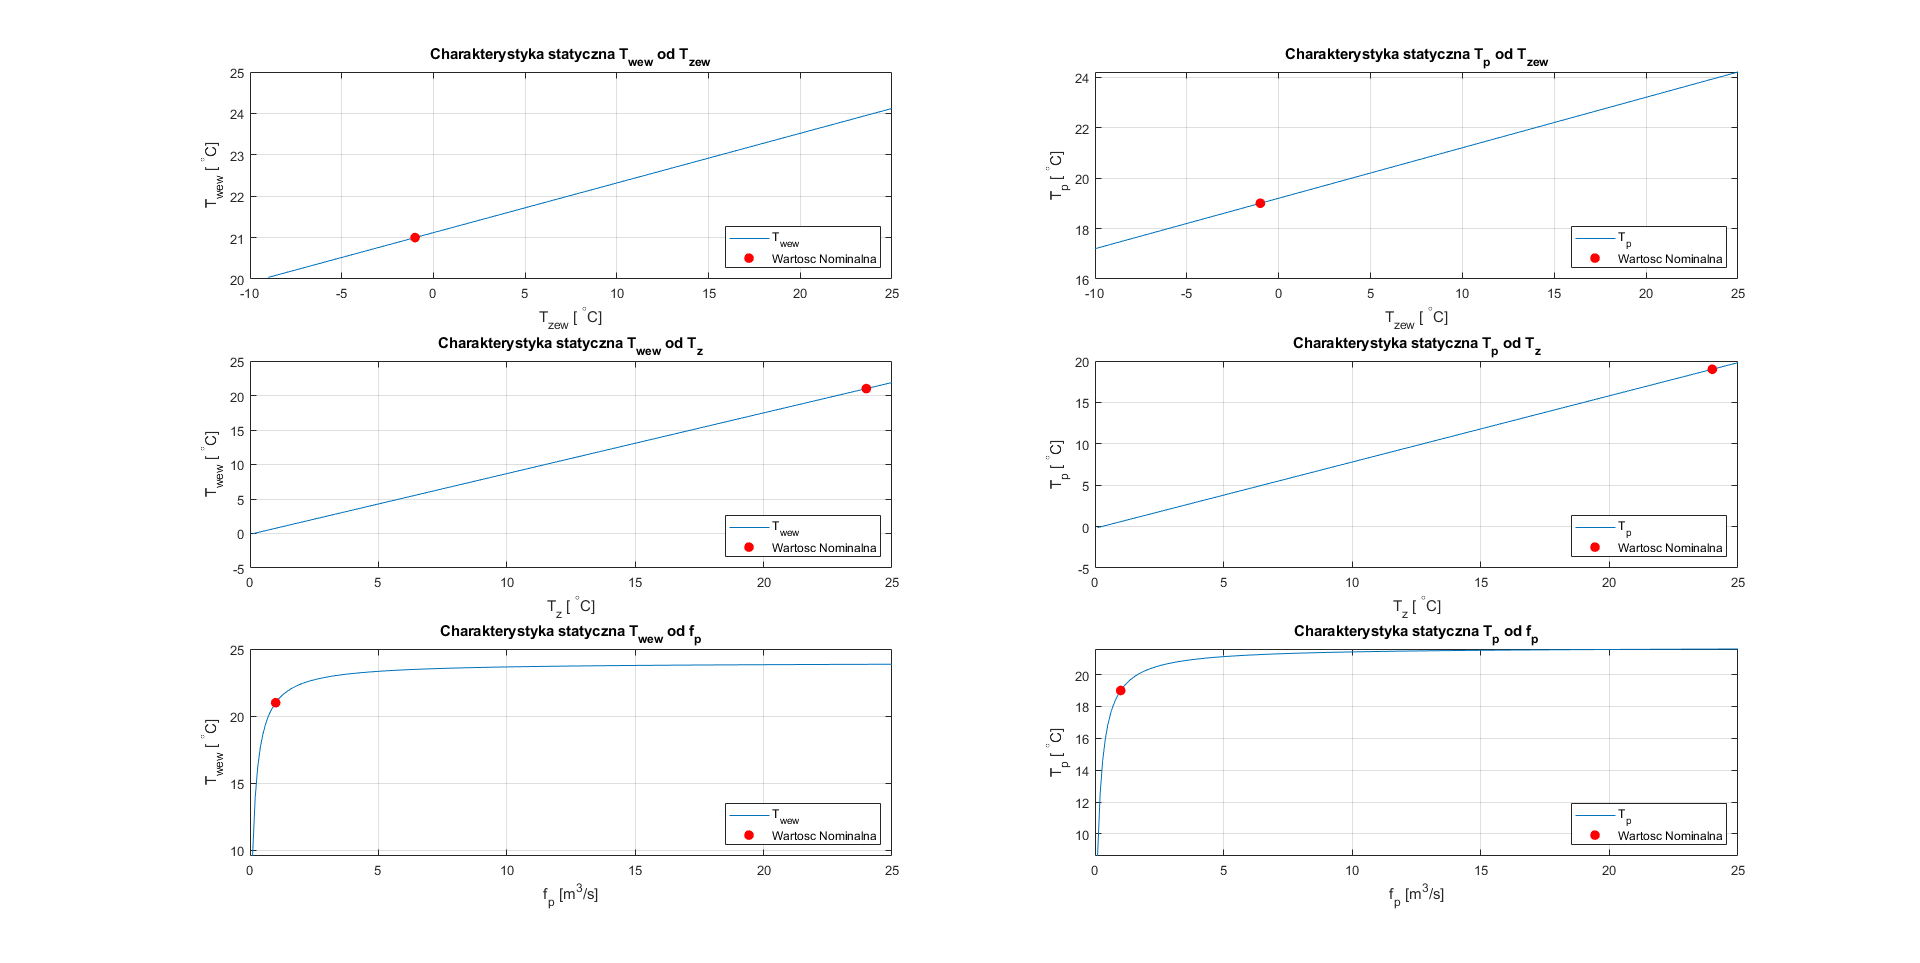
\includegraphics[scale=0.44, center]{statyczne.png}
    \caption{Charakterystyki statyczne}
    \label{plot:statyczne}
    % \hspace\cdot {-8cm} 
\end{figure}

\newpage
% %%%%%%%%%%%%%%%%%%%%%%%%%%%%%%%%%%%%%%%%%%%%%%%%%%%%%%%%%%%%%%%%%%%%%%%%%%%%%% 
\section{Odpowiedzi skokowe modelu nieliniowego}
% \vspace{-1ex}
\begin{figure}[h!]
    \centering
    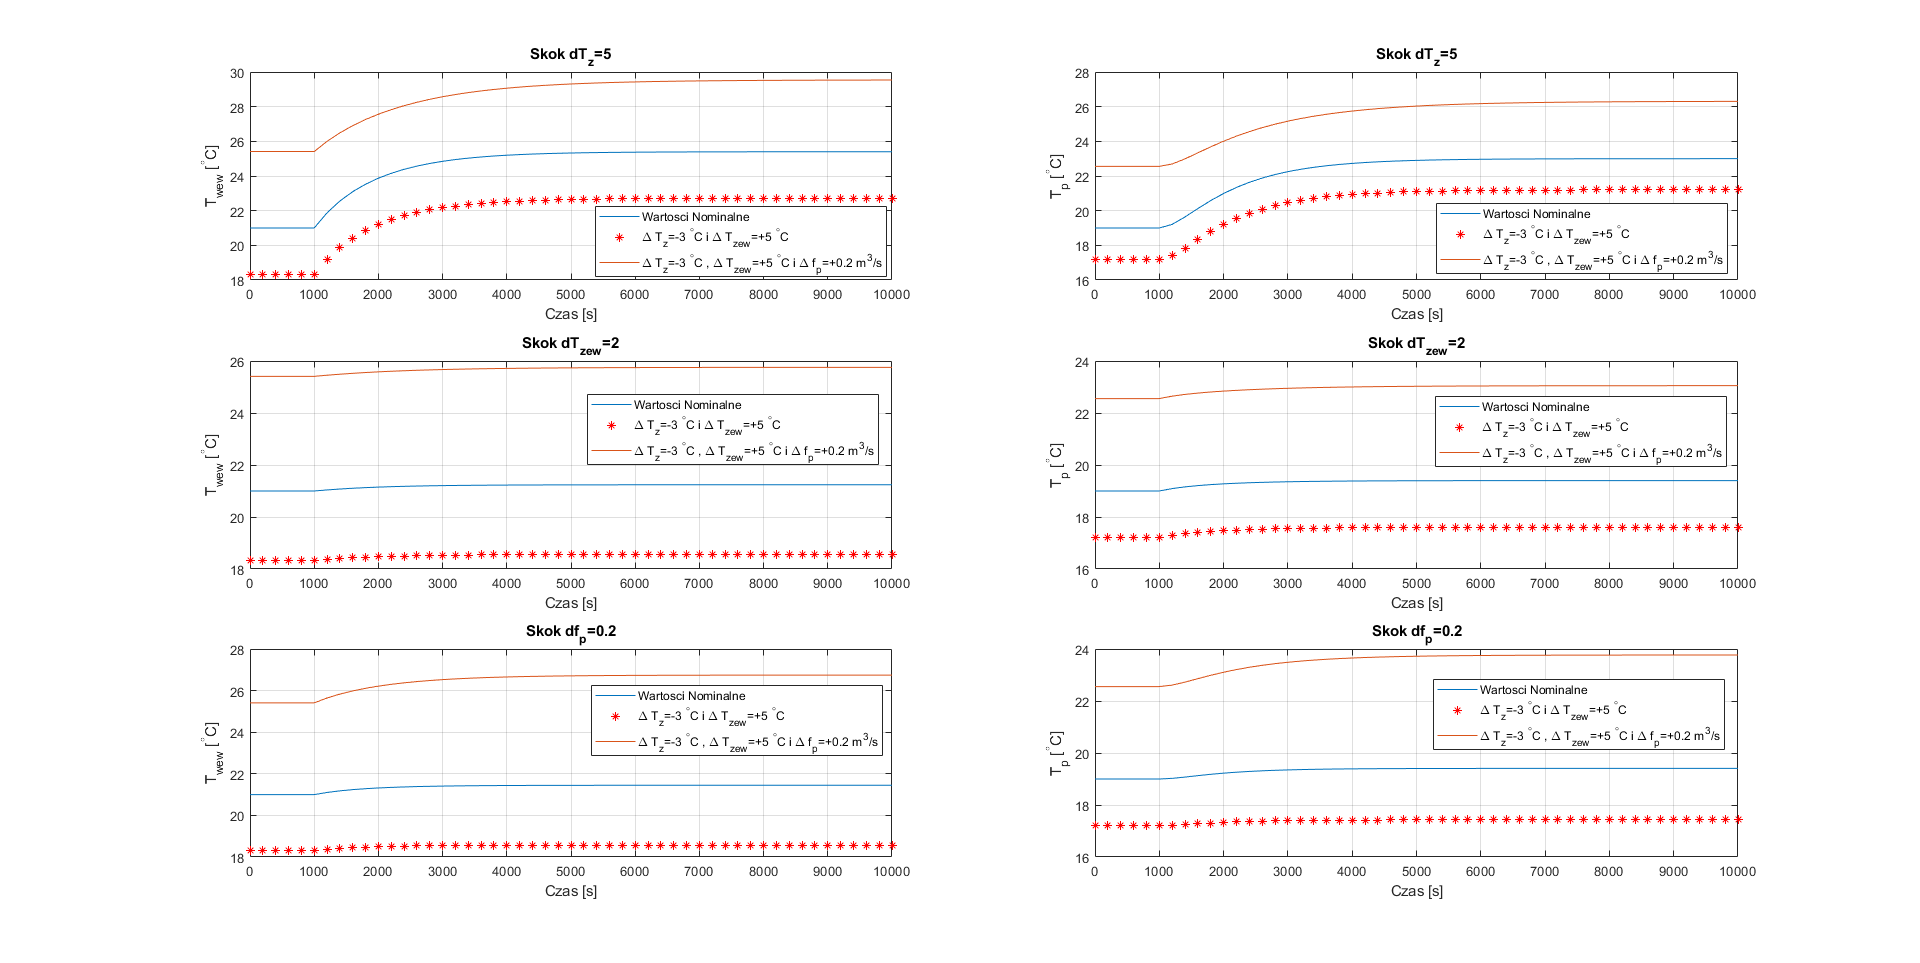
\includegraphics[scale=0.52,center]{skoki_bloki.png}
    \caption{Odpowiedzi skokowe modelu nieliniowego, dla trzech różnych punktów pracy}
    \label{plot:skoki_nl}
\end{figure}


\newpage

\section{Porównanie odpowiedzi skokowych modelu nieliniowego}
Można porównać odpowiedzi skokowe sprowadzając je wszystkie do jednego poziomu:

\begin{figure}[h!]
    \centering
    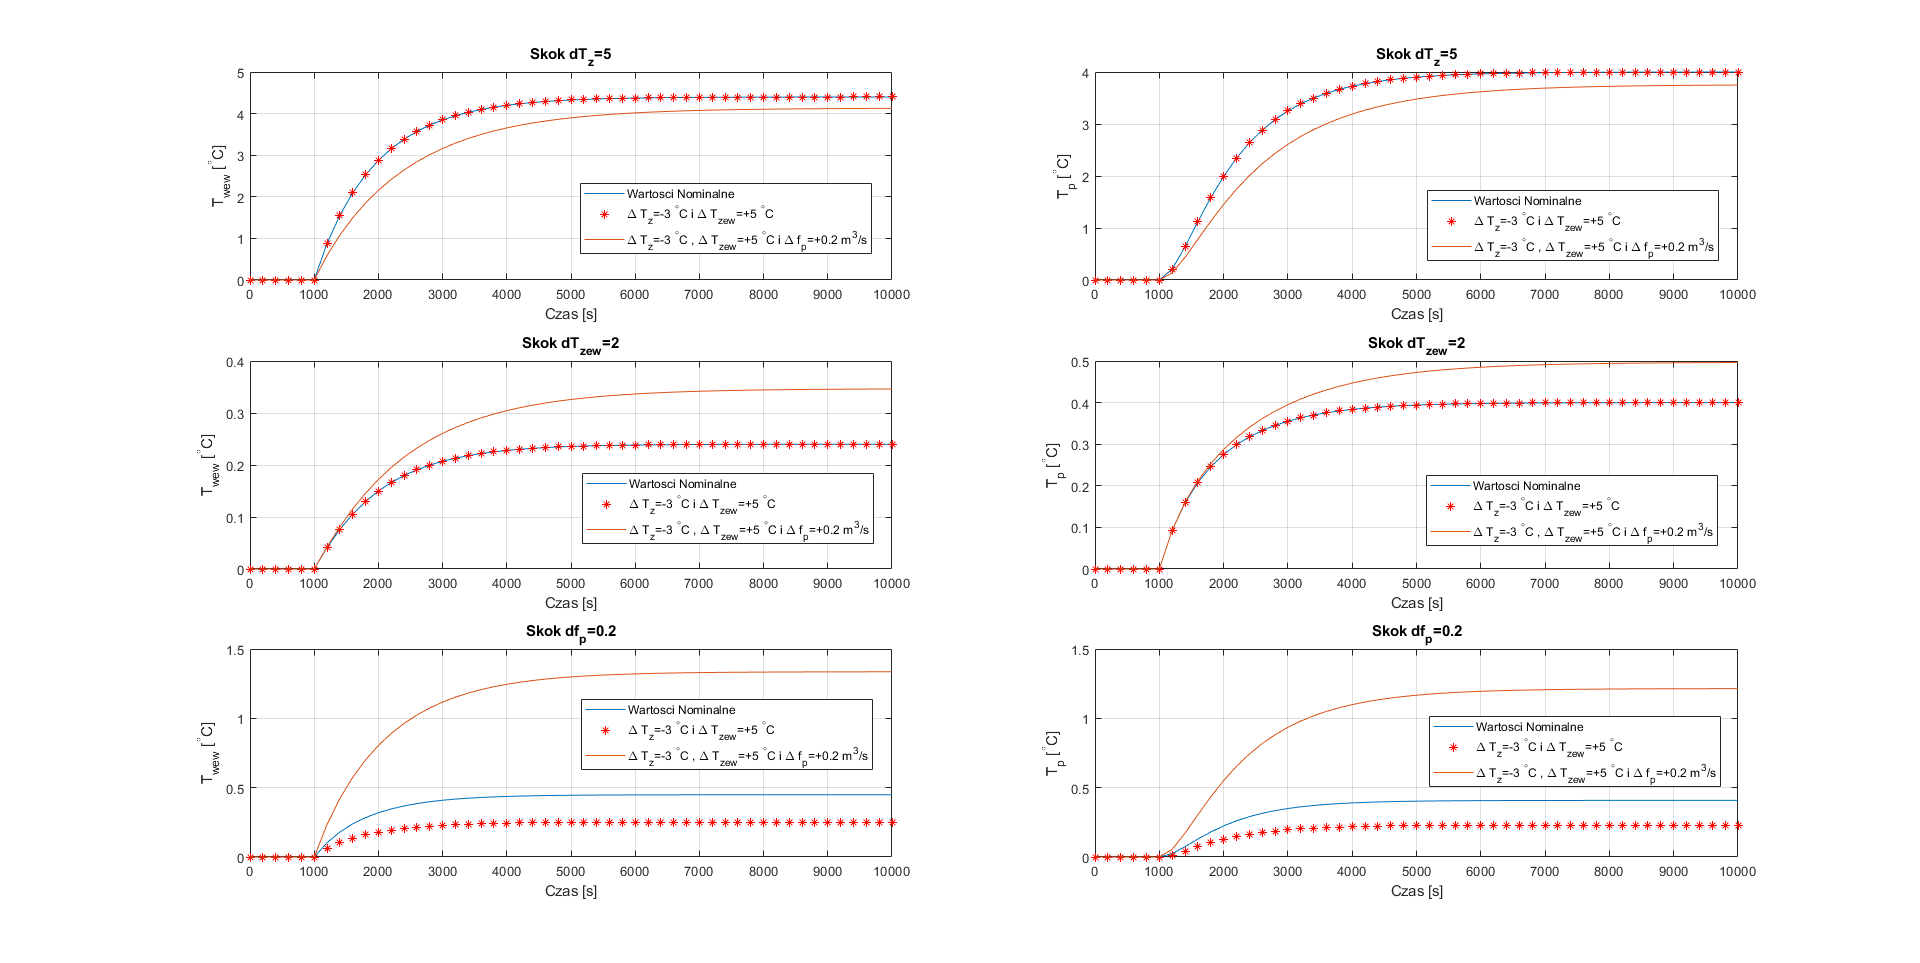
\includegraphics[scale=0.52,center]{leveled_NL.png}
    \caption{Odpowiedzi skokowe modelu nieliniowego, zrównane do tego samego poziomu}
    \label{plot:skoki_nl_leveled}
\end{figure}
% W modelu nieliniowym odpowiedź skokowa i czas w którym układ się stabilizuje zależy od punktu pracy. Wykresy potwierdzają, że nieliniowość (zmiana przepływu) zmienia reakcję obiektu.

%%%%%%%%%%%%%%%%%%%%%%%%%%%%%%%%%%%%%%%%%%%%%%%%%%%%%%%%%%%%%%%%%%%%%%%%%%%%%% 

\newpage


\section{Odpowiedzi skokowe modeli liniowych}
Tworzenie równań potrzebnych do modelu State Space:
% Po przekształceniu oryginalnych równań i ich zlinearyzowaniu otrzymujemy macierze, których używamy w module State Space:
% %%%%%%%%%%%%%%%%%%%%%%%%%%%%%%%%%%%%%%%%%%%%%%%%%%%%%%%%%%%%%%%%%%%%%%%%%%%%%% 
% y = Cx + Du
% x' = Ax + Bu


% x' = Ax + Bu
%-------------------------------------------------
\begin{center}
    \begin{bmatrix}
        \dot{T}_{wew} \\[0.3em]
        \dot{T}_{p}            
    \end{bmatrix}
    =
    \begin{bmatrix}
        \frac{-\Big(c_{p}\cdot \rho_{p} \cdot f_{p} + K_{1} +K_{w} \Big)}{C_{vw}} & \frac{K_{1}}{C_{vw}}  \\[0.3em]
        \frac{K_{1}}{C_{vp}} & \frac{-\Big(K_{1}+K_{p}\Big)}{C_{vp}}           
    \end{bmatrix}
    \begin{bmatrix}
        T_{wew} \\[0.3em]
        T_{p}          
    \end{bmatrix}
    +
    \begin{bmatrix}
        \frac{\Big(c_{p}\cdot \rho_{p} \cdot f_{p} \Big)}{C_{vw}} & \frac{K_{w}}{C_{vw}}  \\[0.3em]
        0 & \frac{K_{p}}{C_{vp}}           
    \end{bmatrix}
    \begin{bmatrix}
        T_{z} \\[0.3em]
        T_{zew}          
    \end{bmatrix}
\end{center}
%-------------------------------------------------1
% y = Cx + Du

\begin{center}
    \begin{bmatrix}
        y_{1} \\[0.3em]
        y_{2}            
    \end{bmatrix}
    =
    \begin{bmatrix}
        1 & 0  \\[0.3em]
        0 & 1           
    \end{bmatrix}
    \begin{bmatrix}
        T_{wew} \\[0.3em]
        T_{p}          
    \end{bmatrix}
    +
    \begin{bmatrix}
        0 & 0  \\[0.3em]
        0 & 0           
    \end{bmatrix}
    \begin{bmatrix}
        T_{z} \\[0.3em]
        T_{zew}          
    \end{bmatrix}
\end{center}


% %%%%%%%%%%%%%%%%%%%%%%%%%%%%%%%%%%%%%%%%%%%%%%%%%%%%%%%%%%%%%%%%%%%%%%%%%%%%%
\begin{figure}[h!]
    \centering
    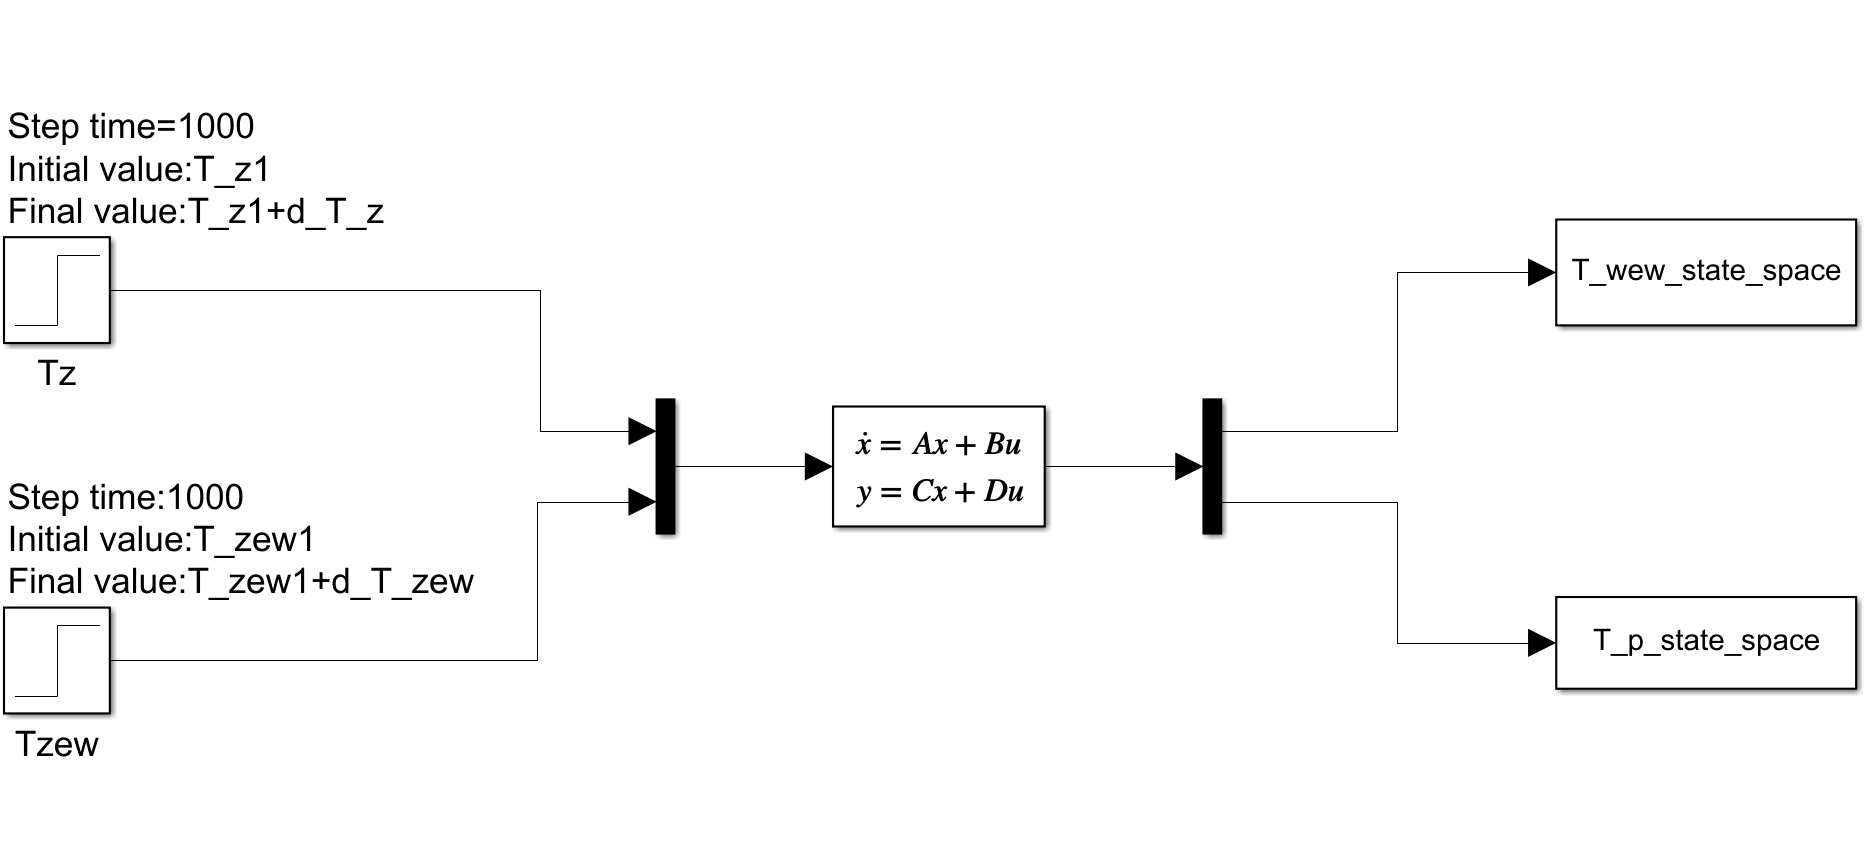
\includegraphics[scale=0.2]{model_state_space.png}
    \caption{Schemat Modelu State Space}
    \label{model:state_space}
\end{figure}

% %%%%%%%%%%%%%%%%%%%%%%%%%%%%%%%%%%%%%%%%%%%%%%%%%%%%%%%%%%%%%%%%%%%%%%%%%%%%%% 
Tworzenie transmitancji na podstawie State Space'a za pomocą funkcji MATLAB'a:\\
% Funkcja ktora zamienia state space na transmitancje

\begin{center}
    \text{[ L1, M1 ] = ss2tf(A,B,C,D,1)}\\
    \text{[ L2, M2 ] = ss2tf(A,B,C,D,2)}
\end{center}

% TRANSMITANCJA
\begin{figure}[h!]
    \centering
    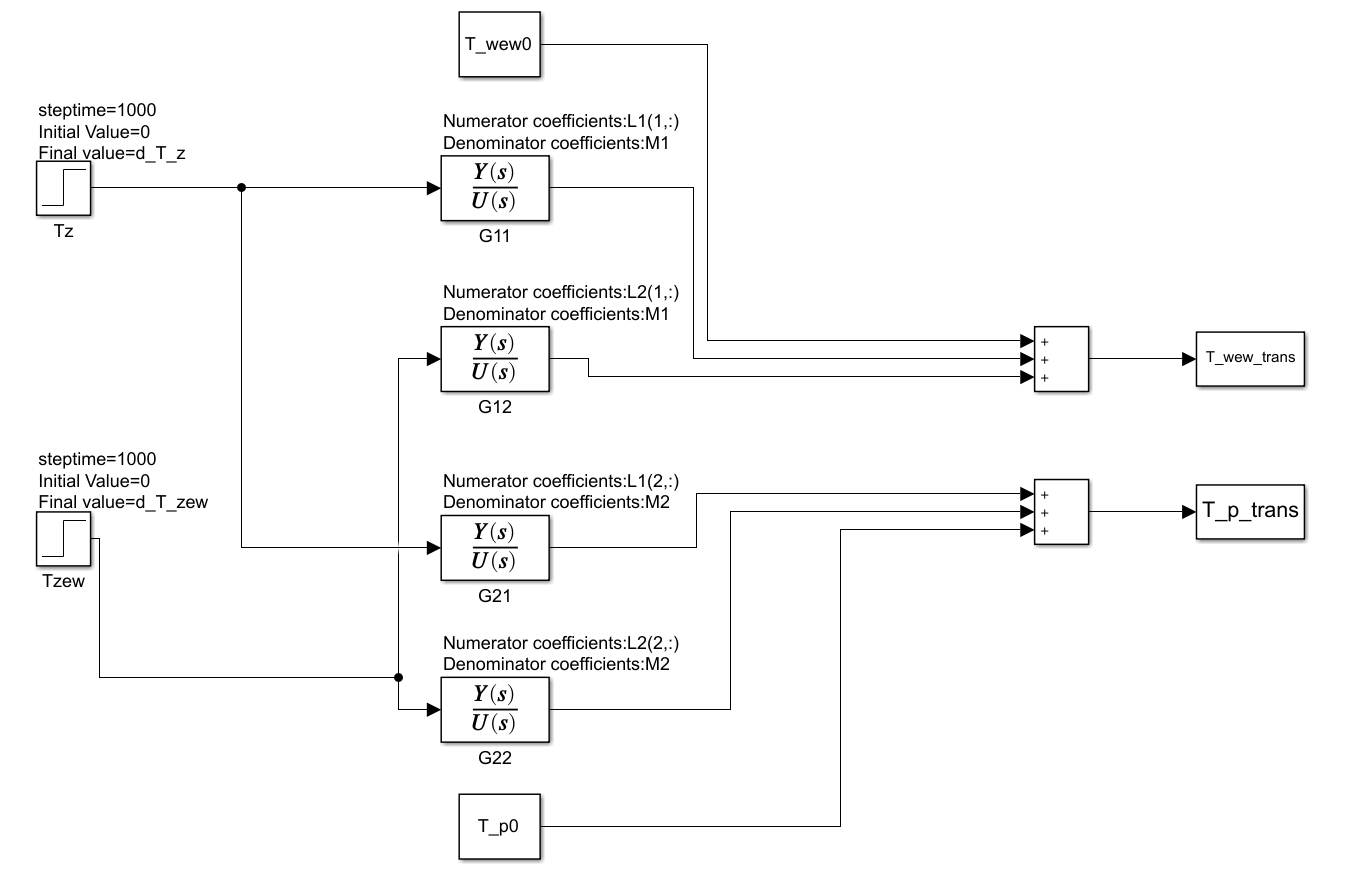
\includegraphics[scale=0.31]{model_transmitancja.png}
    \caption{Schemat Modelu Transmitacyjnego}
    \label{model:trans}
\end{figure}{}
% %%%%%%%%%%%%%%%%%%%%%%%%%%%%%%%%%%%%%%%%%%%%%%%%%%%%%%%%%%%%%%%%%%%%%%%%%%%%%


\newpage


\begin{figure}[h!]
    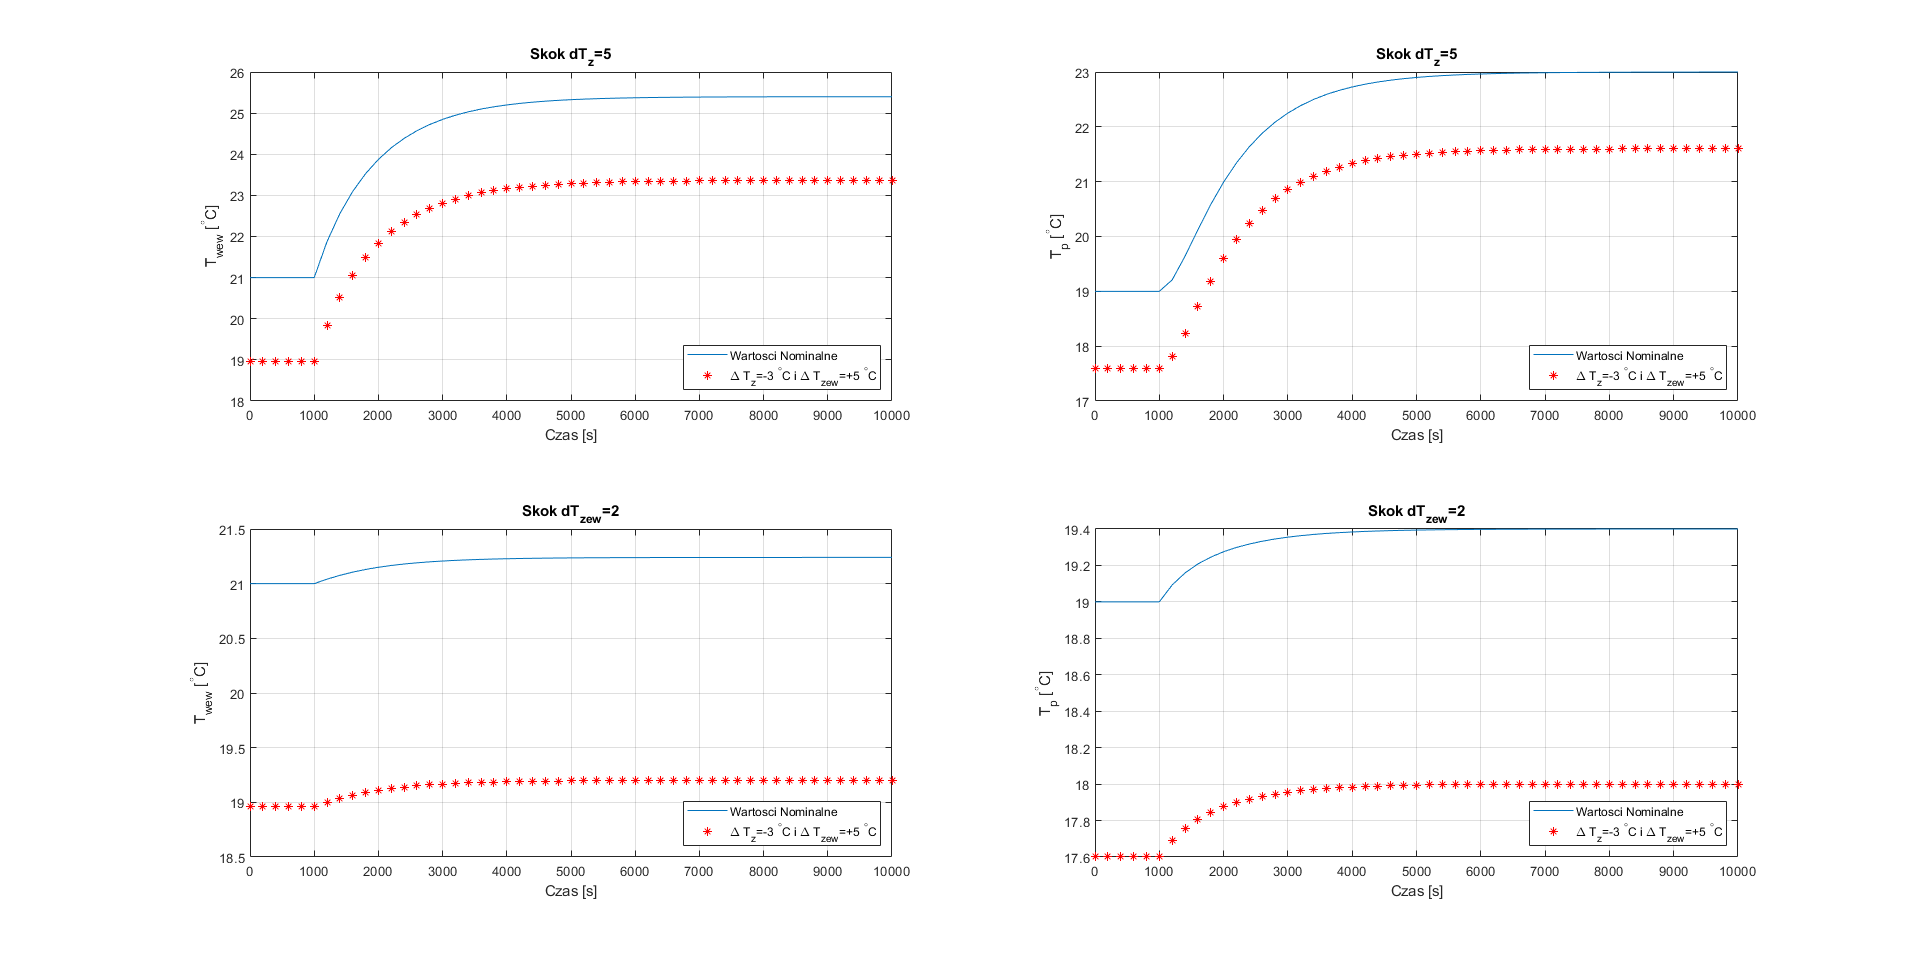
\includegraphics[scale=0.393, center]{skoki_state_space.png}
    \caption{Odpowiedzi skokowe modelu liniowego state space, dla dwóch różnych punktów pracy}
    \label{plot:state_space_skoki}
    \centering
\end{figure}{}



\begin{figure}[h!]
    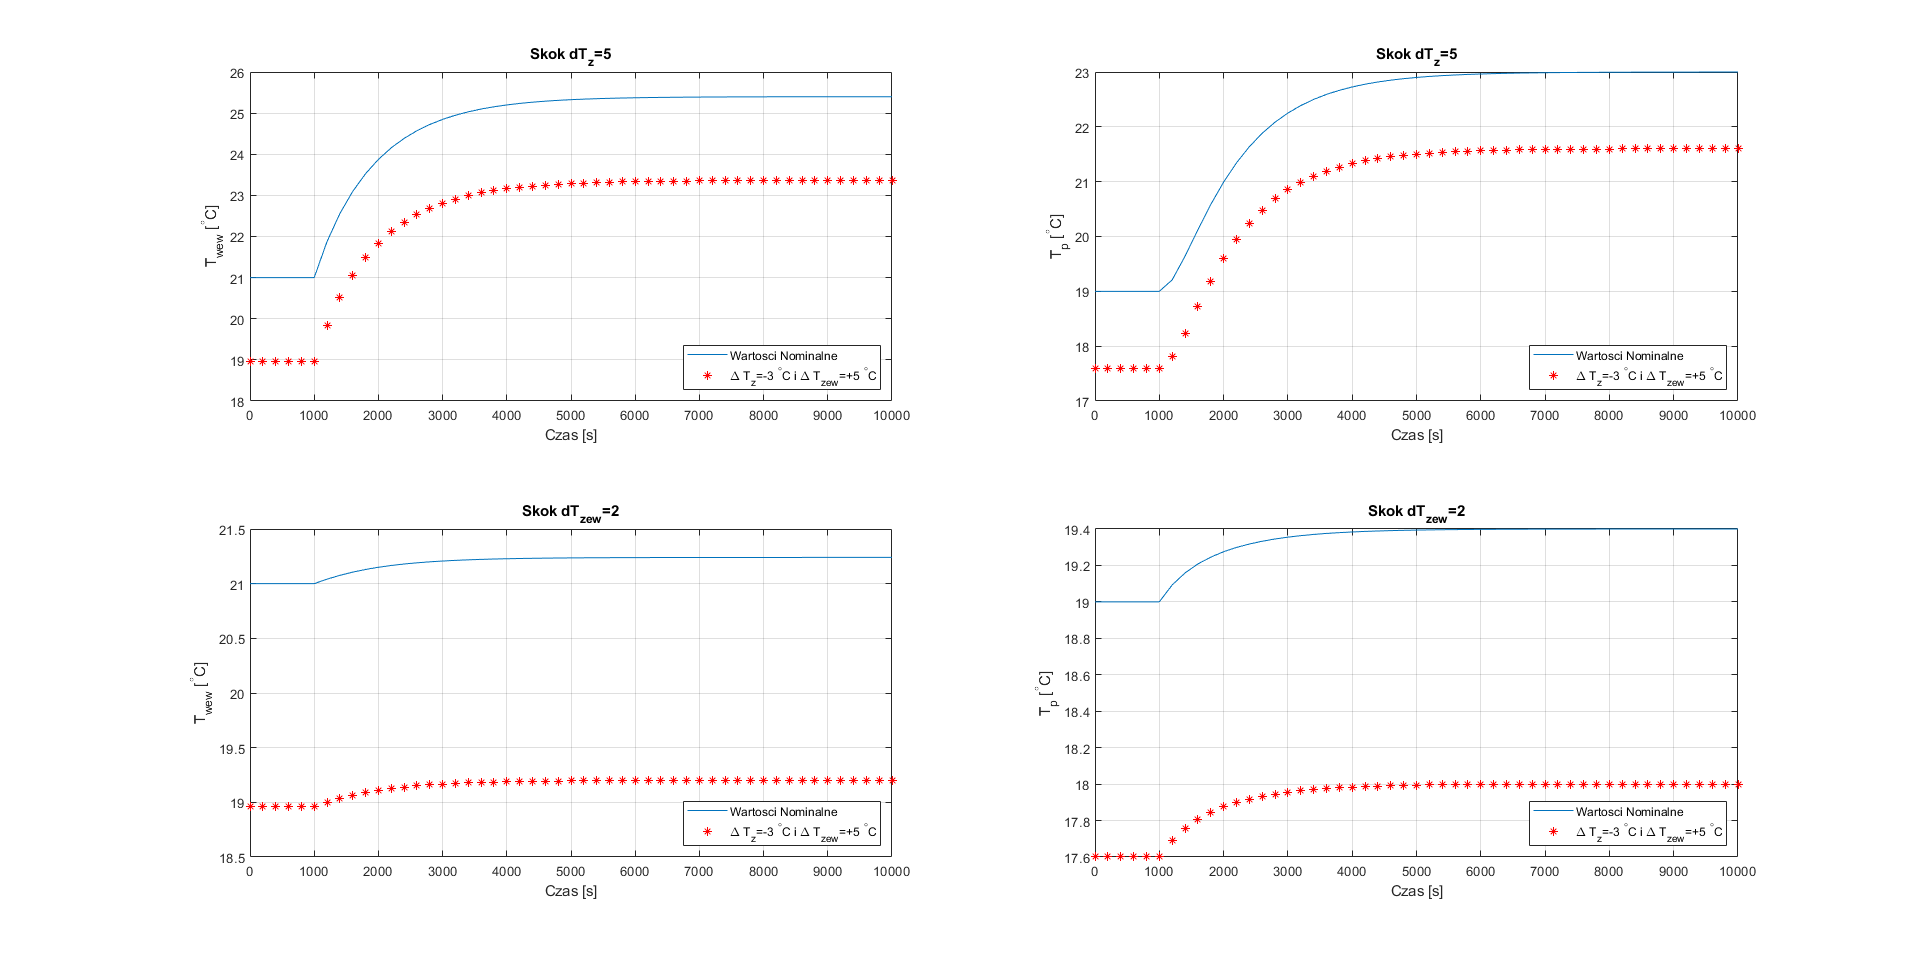
\includegraphics[scale=0.39, center]{skoki_state_space.png}
    \caption{Odpowiedzi skokowe modelu liniowego transmitancji, dla dwóch różnych punktów pracy}
    \label{plot:trans_skoki}
    \centering
\end{figure}{}

% %%%%%%%%%%%%%%%%%%%%%%%%%%%%%%%%%%%%%%%%%%%%%%%%%%%%%%%%%%%%%%%%%%%%%%%%%%%%%

\newpage

\begin{figure}[h!]
    \centering
    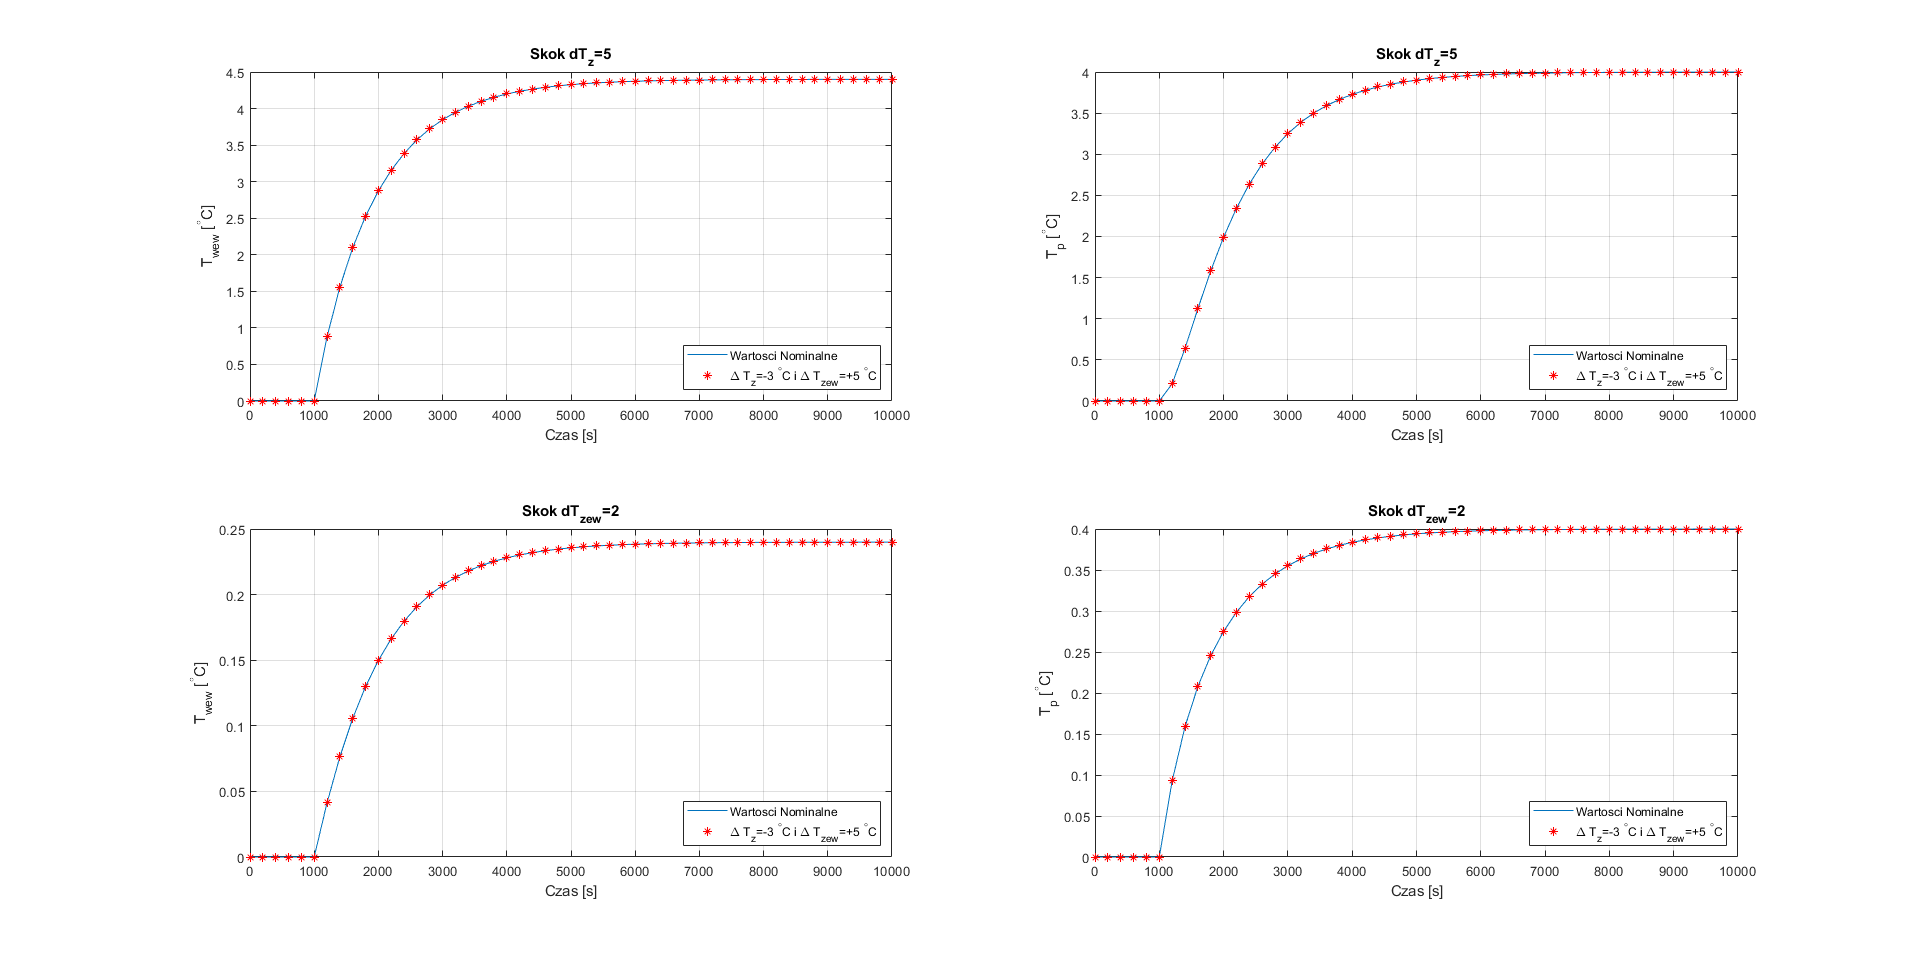
\includegraphics[scale=0.393, center]{leveled_state_space.png}
    \caption{Sprowadzone do tego samego poziomu odpowiedzi skokowe modelu ze State Space}
    \label{plot:state_space_skoki_leveled}
\end{figure}{}


\begin{figure}[h!]
    \centering
    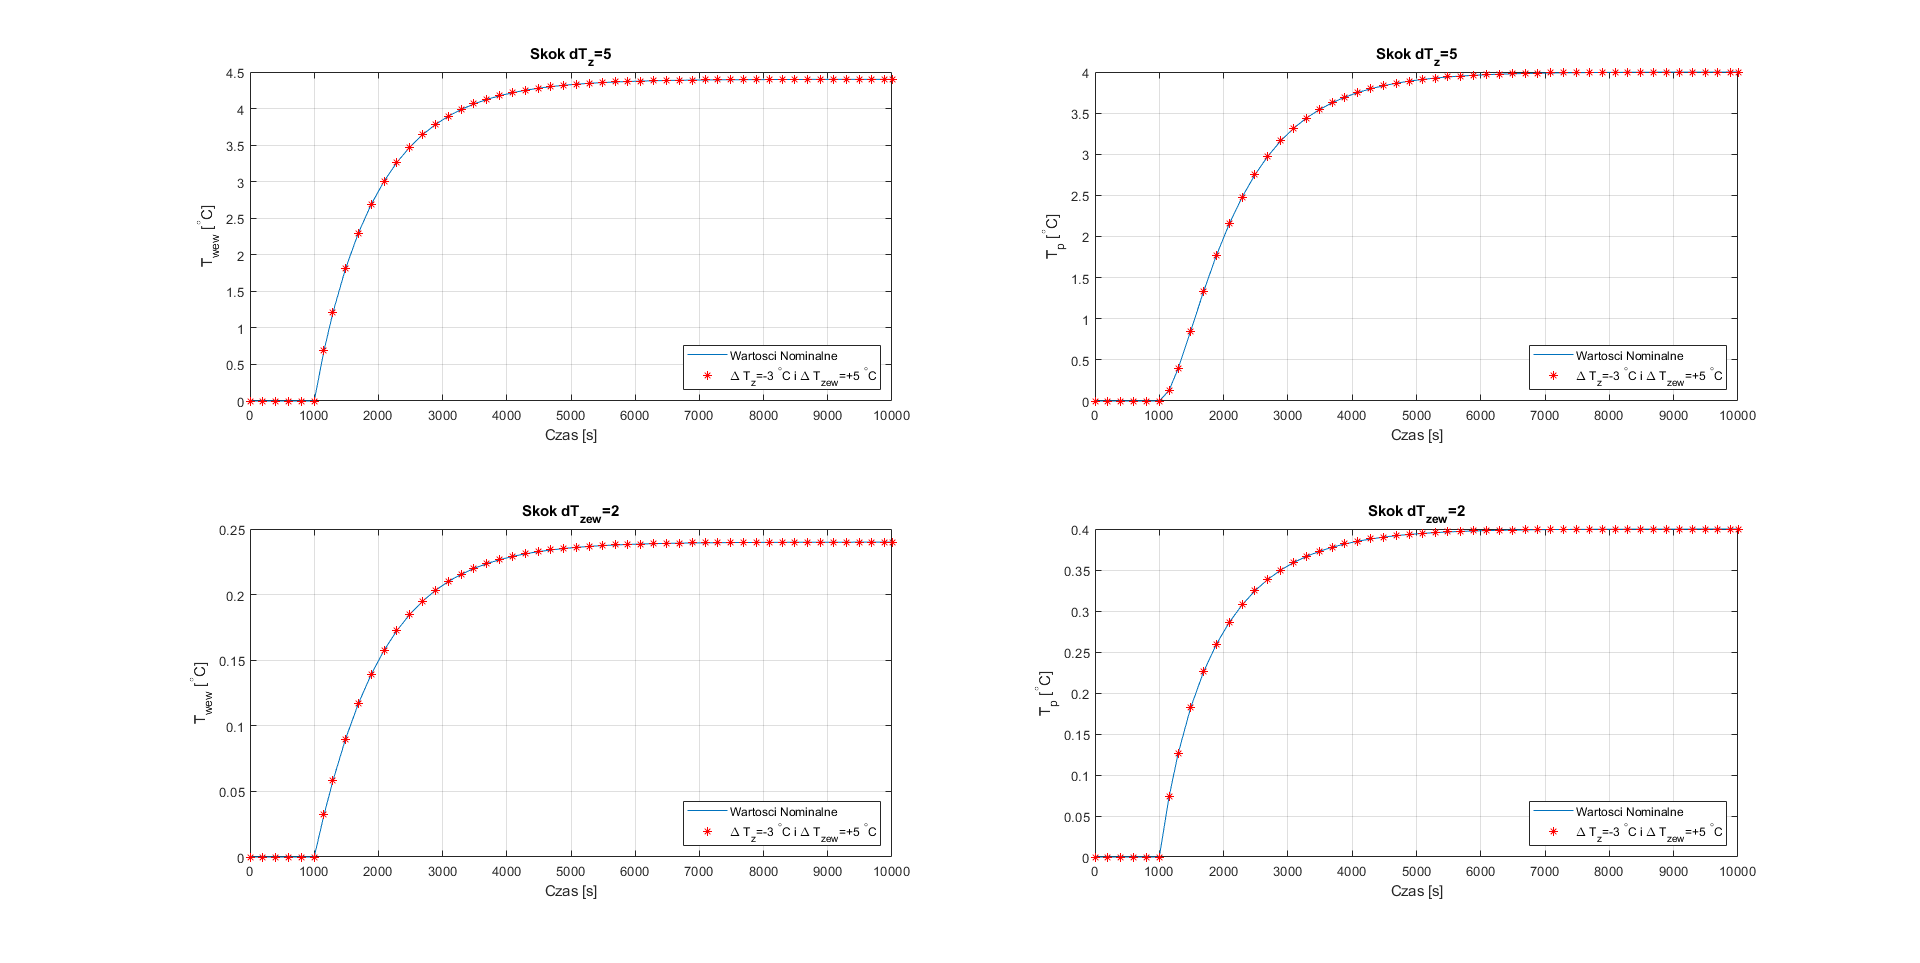
\includegraphics[scale=0.39, center]{leveled_transmitancja.png}
    \caption{Sprowadzone do tego samego poziomu odpowiedzi skokowe modelu z Transmitancją}
    \label{plot:trans_skoki_leveled}
\end{figure}{}

% \begin{}[h!]
% Po przyrównaniu ze do jednego poziomu odpowiedzi skokowych modeli wykorzystujących State Space oraz Transmitancję jasno widać, że w związku z brakiem zmiany $f_{p}$ reakcje obiektu pomimo różnych punktów pracy (gdzie State Space'owi oraz Transmitancji zadano tą samą parę punktów pracy) są takie same.
% \end{}
% %%%%%%%%%%%%%%%%%%%%%%%%%%%%%%%%%%%%%%%%%%%%%%%%%%%%%%%%%%%%%%%%%%%%%%%%%%%%%
\section{Wnioski}

Na rysunku \ref{model:NL} znajduje się model nieliniowy obiektu z rysunku \ref{fig:domek_rysunek}. Jego odpowiedzi skokowe na rysunku \ref{plot:skoki_nl} przy trzech różnych punktach pracy opisanych w legendzie, pierwszym są wartości nominalne, w drugim zmniejszamy $T_{z}$ o 3 $^{\circ}C$  oraz zwiększamy $T_{zew}$ o 5 $^{\circ}C$, w trzecim punkcie pracy oprócz tego co jest w drugim dodatkowo zwiększamy $f_{p}$ o $0.2$ $\frac{m^3}{s}$.
Na rysunku \ref{plot:skoki_nl_leveled}, otrzymane wykresy zostały zrównane do jednego poziomu, dla jednakowych wartości siły nawiewu wykresy mają identyczny przebieg. Co oznacza, że szybkość zmian temperatur zależy od $f_{p}$.\\
% jak różnią się między sobą odpowiedzi skokowe układu przy różnych punktach pracy. Widać wyrazie jak zmiana $f_{p}$ zmienia odpowiedź skokową.
Następnym etapem jest stworzenie modelu State Space (rysunek \ref{model:state_space}) oraz Transmitancji (rysunek \ref{model:trans}), którą możemy uzyskać odpowiednim poleceniem Matlaba z macierzy użytych do stworzenia State Space.
Dla modelu liniowego State Space na rysunku \ref{plot:state_space_skoki} widzimy odpowiedzi skokowe, dla dwóch punktów pracy, gdzie pierwszym jest nominalny, a w drugim zmniejszamy $T_{z}$ o 3 $^{\circ}C$ oraz zwiększamy $T_{zew}$ o 5 $^{\circ}C$. Tak samo postępujemy z drugim modelem liniowym (Transmitancją), której odpowiedzi są widoczne na rysunku \ref{plot:trans_skoki}. Po zrównaniu wykresów obu modeli (rysunki \ref{plot:state_space_skoki_leveled} i \ref{plot:trans_skoki_leveled}) można jasno zaobserwować, że wykresy są takie same. Czas stabilizacji nie zmienia się ponieważ $f_{p}$ jest stałe. Stabilizacja zachodzi powoli z uwagi na dobrane parametry K.

% %%%%%%%%%%%%%%%%%%%%%%%%%%%%%%%%%%%%%%%%%%%%%%%%%%%%%%%%%%%%%%%%%%%%%%%%%%%%%

\section{Załączniki}
Wyprowadzenia:\\
Współczynniki K należy obliczyć podstawiając za pochodne zera, a za pozostałe wartości znane nam wartości nominalne. Otrzymujemy takie oto równanie:
% %%%%%%%%%%%%%%%%%%%%%%%%%%%%%%%%%%%%%%%%%%%%%%%%%%%%%%%%%%%%%%%%%%%%%%%%%%%%%
$$
K_{p}=0.25\cdot K_{w}
$$
\[\begin{cases}
    0 = c_{p}\rho_{p}f_{pN}\Big( T_{zN}-T_{wewN}\Big)-K_{1} \Big(T_{wewN}-T_{pN}\Big)-K_{w}\Big( T_{wewN}-T_{zewN}\Big)      \\
    0 =K_{1}\Big( T_{wewN}-T_{pN}\Big)-K_{p}\Big( T_{pN}-T_{zewN}\Big)  
\end{cases}\]
% %%%%%%%%%%%%%%%%%%%%%%%%%%%%%%%%%%%%%%%%%%%%%%%%%%%%%%%%%%%%%%%%%%%%%%%%%%%%%

\[\begin{cases}
    c_{p}\rho_{p}f_{pN}\Big( T_{zN}-T_{wewN}\Big) = K_{1} \Big(T_{wewN}-T_{pN}\Big) \qquad \ +K_{w}\Big( T_{wewN}-T_{zewN}\Big)      \\
    \qquad \qquad 0 \qquad \qquad =K_{1}\Big( T_{wewN}-T_{pN}\Big)-0.25\cdot K_{w}\Big( T_{pN}-T_{zewN}\Big)
\end{cases}\]
% %%%%%%%%%%%%%%%%%%%%%%%%%%%%%%%%%%%%%%%%%%%%%%%%%%%%%%%%%%%%%%%%%%%%%%%%%%%%%
\[\begin{cases}
    c_{p}\rho_{p}f_{pN}\Big( T_{zN}-T_{wewN}\Big) = K_{1} \Big(T_{wewN}-T_{pN}\Big) \ +K_{w}\Big( T_{wewN}-T_{zewN}\Big)      \\
    K_{1}=\frac{0.25\cdot K_{w}\Big( T_{pN}-T_{zewN}\Big)}{\Big( T_{wewN}-T_{pN}\Big)} 
\end{cases}\]
% %%%%%%%%%%%%%%%%%%%%%%%%%%%%%%%%%%%%%%%%%%%%%%%%%%%%%%%%%%%%%%%%%%%%%%%%%%%%%
Rozwiązanie Analityczne: 
\[\begin{cases}
     K_{w} =\frac{c_{p}\rho_{p}f_{pN}\Big( T_{zN}-T_{wewN}\Big)}{0.25\cdot \Big( T_{pN}-T_{zewN}\Big) \ +\Big( T_{wewN}-T_{zewN}\Big)}     \\
    K_{1}=\frac{0.25\cdot K_{w}\Big( T_{pN}-T_{zewN}\Big)}{\Big( T_{wewN}-T_{pN}\Big)} 
\end{cases}\]
% %%%%%%%%%%%%%%%%%%%%%%%%%%%%%%%%%%%%%%%%%%%%%%%%%%%%%%%%%%%%%%%%%%%%%%%%%%%%%
\begin{center}
    \begin{bmatrix}
        c_{p}\rho_{p}f_{pN}\Big( T_{zN}-T_{wewN}\Big) \\[0.3em]
        0            
    \end{bmatrix}
    =
    \begin{bmatrix}
        \Big(T_{wewN}-T_{pN}\Big) & \Big( T_{wewN}-T_{zewN}\Big)  \\[0.3em]
        \Big( T_{wewN}-T_{p}\Big) & -0.25\Big( T_{pN}-T_{zewN}\Big)          
    \end{bmatrix}
    \begin{bmatrix}
        K_{1} \\[0.3em]
        K_{w}           
    \end{bmatrix}
\end{center}

% %%%%%%%%%%%%%%%%%%%%%%%%%%%%%%%%%%%%%%%%%%%%%%%%%%%%%%%%%%%%%%%%%%%%%%%%%%%%%
\begin{flushleft}
    
Rozwiązanie Macierzowe:
\end{flushleft}{}

% \begin{equation}
\begin{center}
% \begin{flushleft}

    \begin{bmatrix}
        K_{1} \\[0.3em]
        K_{w}           
    \end{bmatrix}
    =
$
\begin{bmatrix}
    \left(T_{wewN}-T_{pN}\right) & \left( T_{wewN}-T_{zewN}\right)  \\[0.3em]
    \left( T_{wewN}-T_{pN}\right) & -0.25\left( T_{pN}-T_{zewN}\right)          
\end{bmatrix}^{-1}
$
    \begin{bmatrix}
        c_{p}\rho_{p}f_{pN}\Big( T_{zN}-T_{wewN}\Big) \\[0.3em]
        0            
    \end{bmatrix}
\end{center}
% \end{flushleft}{}
% %%%%%%%%%%%%%%%%%%%%%%%%%%%%%%%%%%%%%%%%%%%%%%%%%%%%%%%%%%%%%%%%%%%%%%%%%%%%%


Po przekształceniu oryginalnych równań i ich zlinearyzowaniu otrzymujemy macierze, których używamy w module State Space:
% %%%%%%%%%%%%%%%%%%%%%%%%%%%%%%%%%%%%%%%%%%%%%%%%%%%%%%%%%%%%%%%%%%%%%%%%%%%%%% 
% y = Cx + Du
% x' = Ax + Bu

\[\begin{cases}
    C_{vw} \dot{T}_{wew}(t) = c_{p}\rho_{p}f_{p}(t)\Big( T_{z}(t)-T_{wew}(t)\Big)-K_{1} \Big(T_{wew}(t)-T_{p}(t)\Big)-K_{w}\Big( T_{wew}(t)-T_{zew}(t)\Big)      \\
    C_{vp} \dot{T}_{p}(t)=K_{1}\Big( T_{wew}(t)-T_{p}(t)\Big)-K_{p}\Big( T_{p}(t)-T_{zew}(t)\Big)  
\end{cases}\]
% %%%%%%%%%%%%%%%%%%%%%%%%%%%%%%%%%%%%%%%%%%%%%%%%%%%%%%%%%%%%%%%%%%%%%%%%%%%%%%
\[\begin{cases}
    \dot{T}_{wew} =\Big( T_{wew} \Big( c_{p}\rho_{p}f_{p} -K_{1} -K_{w} \Big)+T_{p}\Big( K_{1} \Big) +T_{z}\Big( c_{p}\rho_{p}f_{p}\Big)+ T_{zew}\Big( K_{w} \Big)  \Big)\frac{1}{C_{vw} }    \\
    \dot{T}_{p} = \Big(T_{wew} \Big(K_{1}\Big)-T_{p}\Big( K_{1} +L_{p} \Big)+T_{zew} \Big( K_{p} \Big)\Big)\frac{1}{C_{vp}} 
\end{cases}\]
% x' = Ax + Bu
%-------------------------------------------------
\begin{center}
    \begin{bmatrix}
        \dot{T}_{wew} \\[0.3em]
        \dot{T}_{p}            
    \end{bmatrix}
    =
    \begin{bmatrix}
        \frac{-\Big(c_{p}\cdot \rho_{p} \cdot f_{p} + K_{1} +K_{w} \Big)}{C_{vw}} & \frac{K_{1}}{C_{vw}}  \\[0.3em]
        \frac{K_{1}}{C_{vp}} & \frac{-\Big(K_{1}+K_{p}\Big)}{C_{vp}}           
    \end{bmatrix}
    \begin{bmatrix}
        T_{wew} \\[0.3em]
        T_{p}          
    \end{bmatrix}
    +
    \begin{bmatrix}
        \frac{\Big(c_{p}\cdot \rho_{p} \cdot f_{p} \Big)}{C_{vw}} & \frac{K_{w}}{C_{vw}}  \\[0.3em]
        0 & \frac{K_{p}}{C_{vp}}           
    \end{bmatrix}
    \begin{bmatrix}
        T_{z} \\[0.3em]
        T_{zew}          
    \end{bmatrix}
\end{center}
%-------------------------------------------------1
% y = Cx + Du

\begin{center}
    \begin{bmatrix}
        y_{1} \\[0.3em]
        y_{2}            
    \end{bmatrix}
    =
    \begin{bmatrix}
        1 & 0  \\[0.3em]
        0 & 1           
    \end{bmatrix}
    \begin{bmatrix}
        T_{wew} \\[0.3em]
        T_{p}          
    \end{bmatrix}
    +
    \begin{bmatrix}
        0 & 0  \\[0.3em]
        0 & 0           
    \end{bmatrix}
    \begin{bmatrix}
        T_{z} \\[0.3em]
        T_{zew}          
    \end{bmatrix}
\end{center}

% %%%%%%%%%%%%%%%%%%%%%%%%%%%%%%%%%%%%%%%%%%%%%%%%%%%%%%%%%%%%%%%%%%%%%%%%%%%%%

% Warunki poczatkowe dla syulacji w state space
% wartosci poczatkowe2

\\
\[\begin{cases}
    T_{wew0} = \frac{(c_{p}\cdot \rho_{p} \cdot f_{p}\cdot T_{z}+K_{1}\cdot K_{p}\cdot T_{zew}\cdot (K_{1}+K_{p}) +K_{w}\cdot T_{zew})}{(c_{p}\cdot \rho_{p}\cdot f_{p}+K_{1}+K_{w}-(K_{1}^{2})\cdot (K_{1}+K_{p}))}  \\
    T_{p0} = (K_{1}\cdot T_{wew0}+K_{p}\cdot T_{zew})\cdot (K_{1}+K_{p});

\end{cases}\]

% %%%%%%%%%%%%%%%%%%%%%%%%%%%%%%%%%%%%%%%%%%%%%%%%%%%%%%%%%%%%%%%%%%%%%%%%%%%%%
\\
Kod w matlabie:
\begin{lstlisting}[style=Matlab-editor]
%Obliczanie parametrów oraz wartości poczatkowych
%%%%%%%%%%%%%%%%%%%%%%%%%%%%%%%%%%%%%%%%%%%%%%%%%%%%%%%%%%%%%%%%%
close all;
%%%%%%%%%%%%%%%%%%%%%%%%%%%%%%%%%%%%%%%%%%%%%%%%%%%%%%%%%%%%%%%%%
% NOMINALNE WARTOSCI
T_zewN = -1;  % 'C
T_zN = 24;    % 'C
T_pN = 19;    % 'C
T_wewN = 21;  % 'C
f_pN = 1;     % m^3/s
c_p = 1000; % J/(kg*C)
ro_p = 1.2; % kg/m^3
dl = 20;   % m
szer = 10; % m
h_w = 5;   % m
h_p = 1.5; % m
V_w = dl*szer*h_w;   % m
V_p = dl*szer*h_p/3; % m dach jest ostroslupem
C_vw = c_p*ro_p*V_w;   % J/C
C_vp = c_p*ro_p*V_p;   % J/C
%%%%%%%%%%%%%%%%%%%%%%%%%%%%%%%%%%%%%%%%%%%%%%%%%%%%%%%%%%%%%%%%%
% Do zmniejszenia zapisu
a=c_p*ro_p*f_pN;
% Pro_porcja K
p=0.25;
% Obliczanie wspolczynnikow K
A = [(T_wewN-T_pN), (T_wewN-T_zewN); 
     (T_wewN-T_pN), (-p*(T_pN-T_zewN))];
B = [a*(T_zN-T_wewN); 0];
K_matrix = inv(A)*B;
% Wspolczynniki przenikalnosci cieplnej K
K_1=K_matrix(1,1); % W/C
K_w=K_matrix(2,1); % W/C
K_p=p*K_w;         % W/C
%%%%%%%%%%%%%%%%%%%%%%%%%%%%%%%%%%%%%%%%%%%%%%%%%%%%%%%%%%%%%%%%%
T_z1 = T_zN;
T_zew1= T_zewN;
f_p1 = f_pN;
% Sprawdzenie "Prostej kreski"
% Warunki poczatkowe
T_wew0 = T_wewN
T_p0=T_pN
% Wartosci skok�w w step'ach
steptime=1000;
d_T_z = 0;
d_f_p = 0;
d_T_zew = 0;
% Warunki poczatkowe dla syulacji w state space
% wartosci poczatkowe2
T_zew1 = T_zewN;                                                   
T_wew1 = T_wewN;                                                   
T_p1 = T_pN;                                                     
f_p1 = f_pN;
T_z1 = T_zN;                                                     
M=1/(K_1+K_p);
T_wew0 = (c_p*ro_p*f_p1*T_z1+K_1*K_p*T_zew1*M +K_w*T_zew1)/(c_p*ro_p*f_p1+K_1+K_w-(K_1^2)*M);  
T_p0 = (K_1*T_wew0+K_p*T_zew1)*M;

%Przykład symulacji (test prostej kreski)
steptime=1000;
d_T_z = 0;
d_f_p = 0;
d_T_zew = 0;
sim('my_dom_model');
% Test prostej kreski
figure
plot(t,T_wew_sym1)
hold on;
plot(t,T_p_sym1)
grid on;
title('Test prostej kreski, NL');
xlabel('Czas [s]')
ylabel("Temperatura [^{\circ}C]")
legend('T_{wew}','T_{p}')

%Zmiana punktow pracy
% Zmienione T_zew, T_z i f_p
% wartosci poczatkowe2
T_zew1 = T_zewN-5;                                                   
T_wew1 = T_wewN;                                                   
T_p1 = T_pN;                                                     
f_p1 = f_pN-0.35;
T_z1 = T_zN+8;                                                  
cfp = c_p*ro_p*f_pN;
M=1/(K_1+K_p);
T_wew0 = (c_p*ro_p*f_p1*T_z1+K_1*K_p*T_zew1*M +K_w*T_zew1)/(c_p*ro_p*f_p1+K_1+K_w-(K_1^2)*M);  
T_p0 = (K_1*T_wew0+K_p*T_zew1)*M;
%-----------------------------------
% T_z
subplot(3,2,1)
d_T_z = 5;
d_T_zew = 0;
d_f_p = 0;
sim('my_dom_model');
plot(t,T_wew_sym1)
xlabel('Czas [s]')
ylabel("T_{wew} [^{\circ}C]")
hold on;
grid on
legend('Wartosci Nominalne','\Delta T_{z}=-3 ^{\circ}C i \Delta T_{zew}=+5 ^{\circ}C','\Delta T_{z}=-3 ^{\circ}C , \Delta T_{zew}=+5 ^{\circ}C i \Delta f_{p}=+0.2 m^3/s')

%Obliczenie wspolczynnikow dla State Space
% x'= Ax + Bu
% y = Cx + Du 
A =[ -(a+K_1+K_w)/C_vw,    K_1/C_vw    ;
          K_1/C_vp    , -(K_1+K_p)/C_vp];
            
B =[ c_p*ro_p*f_pN/C_vw, K_w/C_vw ;
             0        , K_p/C_vp ];
C=[1,0;
   0,1];

D=[0,0;
   0,0];
% Warunki poczatkowe dla syulacji w state space
% wartosci poczatkowe2
T_zew1 = T_zewN+5;                                                   
T_wew1 = T_wewN;                                                   
T_p1 = T_pN;                                                     
f_p1 = f_pN;
T_z1 = T_zN-3;                                                     
M=1/(K_1+K_p);
T_wew0 = (c_p*ro_p*f_p1*T_z1+K_1*K_p*T_zew1*M +K_w*T_zew1)/(c_p*ro_p*f_p1+K_1+K_w-(K_1^2)*M);  
T_p0 = (K_1*T_wew0+K_p*T_zew1)*M;
State_Space_Init=[T_wew0; T_p0];

%Obliczenie Transmitancji
% Funkcja ktora zamienia state space na transmitancje
[L1,M1]=ss2tf(A,B,C,D,1);
[L2,M2]=ss2tf(A,B,C,D,2);
% Badanie modelu skokami
%-----------------------------------
% T_zN
d_T_z = 5; %5
d_T_zew = 0; %2
d_f_p = 0; %0.2

%Przyklad rysowania wszystkich modeli naraz
sim('my_dom_model')
subplot(1,1,1)
plot(t,T_wew_sym1,'-')
hold on;
sim('my_dom_trans')
plot(T_wew_trans,'*')
hold on;
sim('my_dom_state_space')
plot(T_wew_state_space,'o')
hold on
title('Twew od skoku Tz=2')
legend('NL','State Space','Transmitancja')
grid on;

%Przyklad sprowadzenia do tego samego poziomu
% f_p
subplot(3,2,5)
d_T_z = 0;
d_T_zew = 0;
d_f_p = 0.2;
sim('my_dom_model');
plot(t,T_wew_sym1-T_wew_sym1(1,1))
xlabel('Czas [s]')
ylabel("T_{wew} [^{\circ}C]")
grid on
title('Skok df_{p}=0.2')
hold on;

%Przykladowe rysowanie charakterystyki
T_zew1 = T_zewN;                                                   
T_wew1 = T_wewN;                                                   
T_p1 = T_pN;                                                     
f_p1 = f_pN;
T_z1 = T_zN;                                                     
a = c_p*ro_p*f_pN;
M=1/(K_1+K_p);

subplot(325);
f_p1=0.1:0.1:25;
T_wewp = (c_p*ro_p*f_p1*T_z1+K_1*K_p*T_zew1*M +K_w*T_zew1)./(c_p*ro_p*f_p1+K_1+K_w-(K_1^2)*M) ;
T_po = (K_1*T_wewp+K_p*T_zew1)*M;
plot(f_p1,T_wewp);
xlabel('f_pN [m^3/s]');
ylabel('T_{wew} [ ^{\circ}C]');
hold on;
plot(f_pN, T_wewN, 'r.','Markersize',25);
title('Charakterystyka statyczna T_{wew} od f_{p}');
grid on;
legend("T_{wew}","Wartosc Nominalna",'Location','SouthEast')




\end{lstlisting}
% https://ih1.redbubble.net/image.676836586.0183/flat,750x,075,f-pad,750x1000,f8f8f8.jpg

\end{document}
